\section{Secure Software / Software Security}

Durch das Aufkommen des Internets nahm auch die vom \textit{National Institute of Standards and Technology} (NIST) erfassten Vulnerabilities mit hohem Ausmass zu.

\subsection{Most Dangerous Software Errors}
Die 25 häufigsten Schwachstellen können in drei Kategorien eingeteilt werden:
\begin{itemize}
	\item Ausgelöst durch unsichere Wege, in denen die Daten gesendet und empfangen werden. Dazu zählen \textit{SQL Injection}, \textit{OS Command Injection}, \textit{XSS}, \textit{CSRF} und \textit{Open Redirect}.
	\item Ausgelöst durch die unsichere Handhabung von Systemressourcen. Dazu gehören \textit{Classic Buffer Overflow}, \textit{Path Traversal}, \textit{Uncontrolled Format String}, \textit{Potentially Dangerous Function} und \textit{Integer Overflow}.
	\item Ausgelöst durch falsche Verwendung, Missbrauch oder Ignorierung von defensiven Sicherheitsmechanismen. Dazu zählen \textit{Missing Authentication}, \textit{Missing/Incorrect Authorization}, \textit{Hard-Coded Credentials}, \textit{Missing Encryption}, \textit{Reliance on Untrusted Inputs}, \textit{Incorrect Permission Assignment}, \textit{Use of broken or risky Cryptographic algorithm} und \textit{One-Way Hash without Salt}.
\end{itemize}

\subsection{Trinity of Trouble}
Folgende drei Aspekte sind mitunter verantwortlich für diese Schwierigkeiten.
\begin{description}
	\item[Connectivity] Immer mehr Systeme sind über das Internet miteinander verbunden und eröffnen somit neue \textit{Attack Vectors}. \textit{Service Oriented Architecture (SOA)} führt alte Systeme, welche nicht für die Vernetzung vorgesehen wurden, zusammen und veröffentlicht diese.
	\item[Extensibility] Systeme sind erweiterbar, wodurch ein teil der Kontrolle abgegeben wird. Über schlecht gewartete Erweiterungen können so neue Schwachstellen entstehen.
	\item[Complexity] Moderne Software wird immer komplexer. Mit dem Umfang nimmt auch die Fehlerrate quadratisch zu.
\end{description}

\subsection{Bugs + Flaws = Defects}
\begin{description}
	\item[Security Bug] Implementation-level Schwachstelle
	\item[Security Flaw] Design-level Schwachstelle (können selten automatisiert erkannt werden)
	\item[Security Defect] Ruhender defekt in der Software, welcher durch ein Bug oder Flaw ausgelöst wird.
\end{description}

\subsection{Software Artefakte}
Es gibt ein gemeinsames Set von Artefakten, welche unabhängig vom eigentlichen Entwicklungsprozess (Scrum, RUP, XP, \ldots) sind. Diese sind:
\begin{easylist}[itemize]
	& Anforderungen und Use Cases
	& Architektur und Design
	& Testpläne
	& Code
	& Tests und Testresultate
	& Rückmeldung von Kunden
\end{easylist}

\subsection{Drei Säulen der Software Security}

Zu den zentralen drei Säulen gehören \textbf{Risiko Management}, \textbf{Best Practices} und \textbf{Fachwissen}.

\subsubsection{Risiko Management}
Man identifiziert die betroffenen Personen, die technischen Risiken, auch die für das Unternehmen, und priorisiert sie anhand der gewonnenen Informationen. Danach kann eine Strategie zur Minderung entwickelt werden. Nach der Anwendung sollten die Anpassungen auf ihre Wirkung hin überprüft werden.

\begin{figure}[H]
	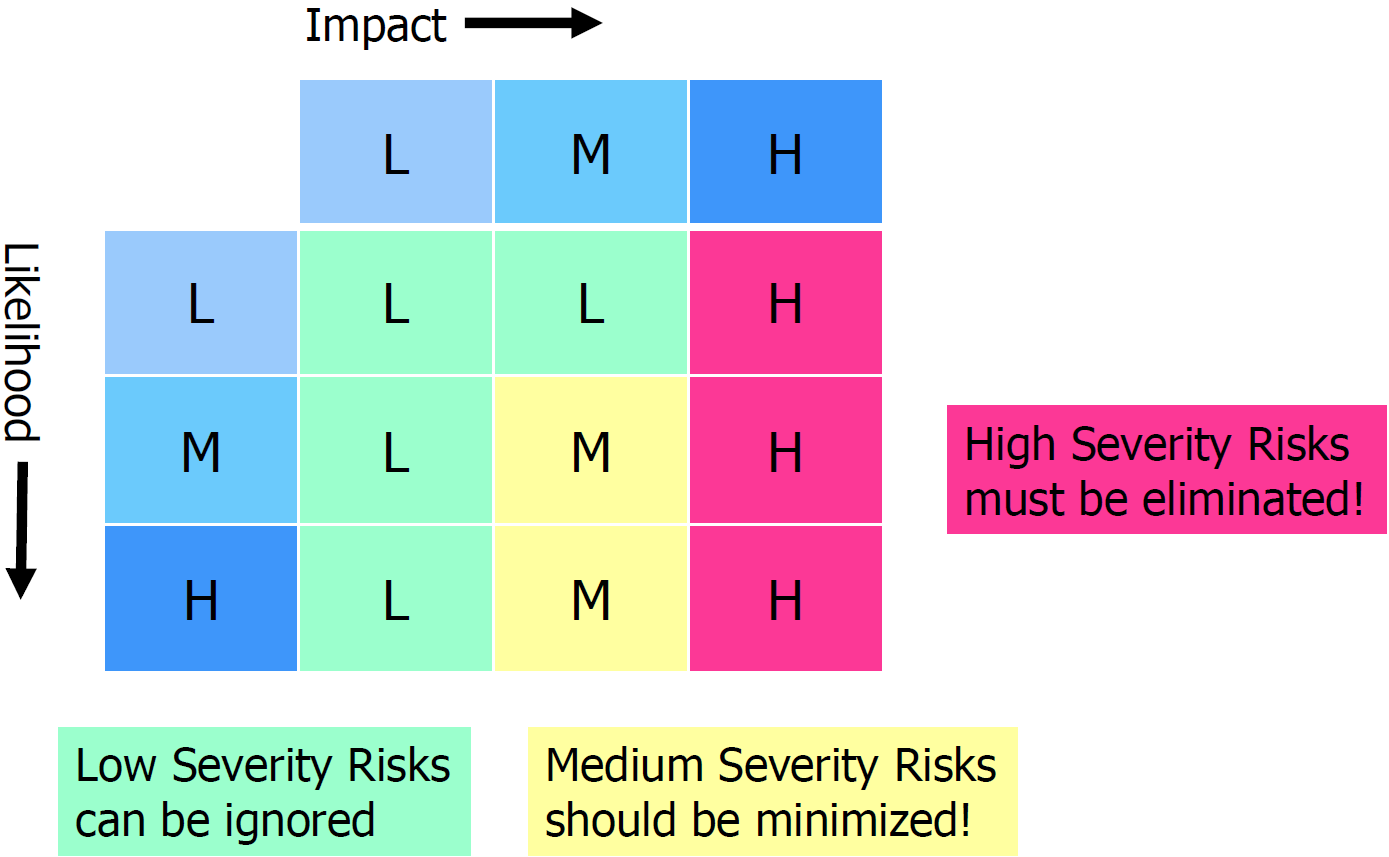
\includegraphics[width=0.6\textwidth]{./img/risk-evaluation}
	\caption{Risiko Evaluations-Matrix}
\end{figure}

\subsubsection{Best Practices}

Es folgen einige Best Practices in der Reihenfolge ihrer Effektivität. Sie können den Kategorien \textbf{K}onstruktiv (white hat) und \textbf{D}estruktiv (black hat) zugeordnet werden.
\begin{easylist}
	& Code Review \textbf{K}
	& Architectural risk analysis (historical knowledge) \textbf{K D}
	& Penetration testing \textbf{D}
	& Risk-based security tests \textbf{D K}
	& Abuse cases \textbf{D K}
	& Security requirements \textbf{K}
	& Security operation \textbf{K}
\end{easylist}

\subsubsection{Fachwissen}
Zum Fachwissen gibt es mehrere Perspektiven. Das Wissen über die Prinzipien, Rahmenbedingungen und Regeln gehören zum Vorgeschriebenen Fachwissen. Dazu gesellt sich die Diagnostischen Fähigkeiten mit dem Wissen über Angriffe, Schwachstellen und Angriffsmuster. Zuletzt benötigt man auch ein Wissen über die Vergangenheit.

\begin{figure}[H]
	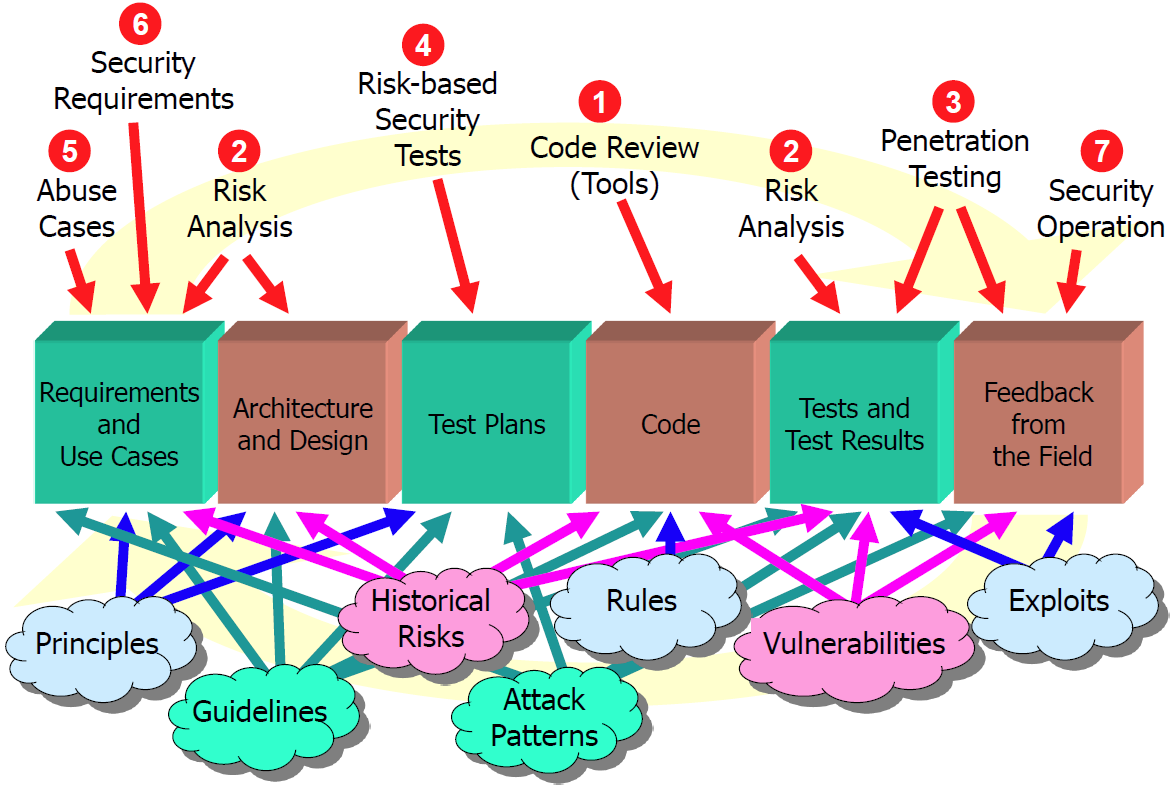
\includegraphics[width=\textwidth]{./img/sdl-best-practice}
	\caption{Best Practices und Fachwissen angewendet auf die Software Artefakte}
\end{figure}

\subsection{Code Analyse}

Für die Analyse von Sourcecode bieten sich mehrere Lösungen an, welche den Quellcode und auch das laufende Programm analysieren und auswerten können. Die ersten Generationen von solchen Analyseprogrammen wurden auch als \textit{Intelligentes Grep} bezeichnet und lieferten viele false positives. In späteren, oft kommerziellen Tools, wurden diese, durch Parsen des Source-Codes, versucht zu minimieren.

Das Wissen aus der Vergangenheit ist in die Regelsätze dieser Software eingeflossen. Jedoch können Probleme in der Softwarearchitektur nicht oder nur selten erkannt werden. Ein manuelles Review ist somit weiterhin nötig. Auch können Abhängigkeiten und falsche Benutzung externer Komponenten nicht korrekt überprüft und erkannt werden.

\subsection{Security Development Lifecycle - SDL}

Der Security Development Lifecycle ist ein Prozess, welcher die \textbf{Sicherheit innerhalb der Softwareentwicklung garantieren} soll. Er wurde von Microsoft entwickelt und gilt als Grundlage, lässt sich also für jede Unternehmensgrösse anpassen. Der SDL umfasst die drei Kernkonzepte \textbf{Schulung}, \textbf{fortwährende Verbesserung der Prozesse} und \textbf{Zurechenbarkeit}.\\
Der SDL sollte auf Projekte mit folgenden Merkmalen angewendet werden:
\begin{easylist}[itemize]
	& Eingesetzt in einem Unternehmen
	& Verarbeitung von personenbezogenen Daten
	& Regelmässige Kommunikation über das Internet oder andere Netzwerke
\end{easylist}
\textbf{Im Prinzip kann der SDL also auf alle Projekte angewendet werden.} Es ist einfacher, diejenigen zu identifizieren, die keinen sicherheitstechnischen Massnahmen benötigen und daher auch auf den SDL verzichten können.\\
Es existieren mehrere Rollen, wovon zwei besonders hervorzuheben sind. Diese lassen sich wiederum weiter unterteilen.
\begin{description}
	\item[Reviewer/Advisory Roles] Diese Rolle soll eine Übersicht über die Sicherheit des Projektes bieten und in der Lage sein, Pläne bezüglich Sicherheit und Datenschutz anzunehmen/abzulehnen. Kann von Internen wie auch externen Personen übernommen werden, aber keine Teammitglieder.
	\item[Team Champions] Diese Rolle ist verantwortlich für den Austausch, Akzeptanz und Verfolgung von minimalen Anforderungen an die Sicherheit und Datenschutz. Sie sind das Gegenstück zu den Advisory Roles und besteht aus Teammitglieder.
\end{description}

Finden die Sicherheitsrelevanten Aktivitäten frühzeitig und innerhalb des Entwicklungsprozesses statt, erhält man den grössten Nutzen daraus.
Um den Microsoft SDL-Prozess einzuhalten müssen die 16 zwingenden Aktivitäten eingehalten werden.

\begin{figure}[H]
	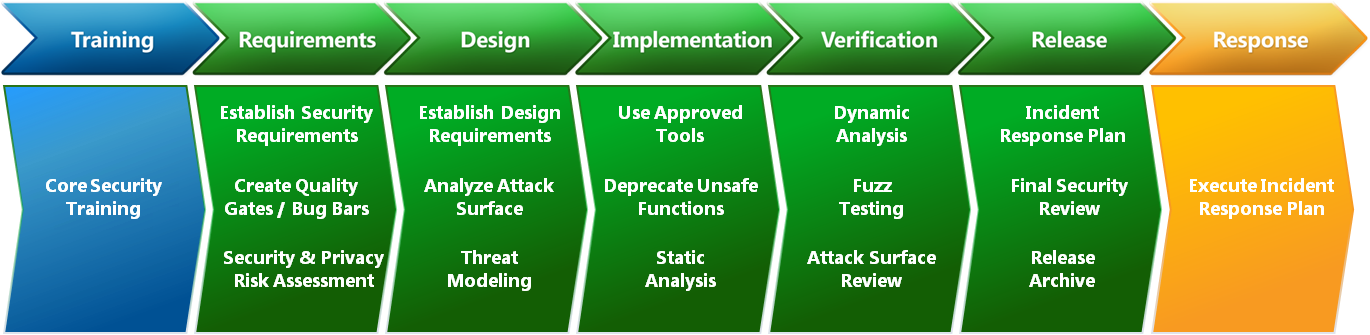
\includegraphics[width=\textwidth]{./img/sdl-overview}
	\caption{Security Development Lifecycle von Microsoft}
\end{figure}

\subsubsection{Training Requirements}
Alle Mitglieder des Entwicklerteams müssen eine Schulung im Bereich Softwaresicherheit erhalten und sich über aktuelle Trends informieren. Die Themen umfassen \textbf{sicheres Design}, \textbf{Modellierung von Bedrohungen}, \textbf{sicheres Coding}, \textbf{Sicherheitstests} und \textbf{Datenschutz}.

\subsubsection{Security Requirements}
Definition von vertrauenswürdigen Anforderungen an das Projekt. Damit können Schlüsselstellen identifiziert werden und die Sicherheit sowie Datenschutz frühzeitig integriert werden. Dies verhindert unnötige Verzögerungen.

\subsubsection{Quality Gates/Bug Bars}
Quality Gates und Bug bars sind minimale Akzeptanzkriterien in Anbetracht der Sicherheit und des Datenschutzes. Das gesamte Team muss sich an die Anforderungen halten, wobei diese nicht dynamisch verändert werden dürfen.
\begin{description}
	\item[Quality Gate] Anforderung an die Code-Qualität bezüglich Compiler-Warnungen, Kommentare, Komplexität, etc.
	\item[Bug Bar] Schwelle für Sicherheitslücken, welche noch im Projekt beim Release enthalten sein dürfen. Z.B. keine Lücken mit der Bewertung "'Kritisch"' oder "'Warnung"'.
\end{description}

\subsubsection{Security and Privacy Risk Assesment}
Beurteilung der Sicherheit- und Datenschutz-Anforderungen von funktionalen Komponenten, welche eine genauere Begutachtung benötigen. Es wird bestimmt, ob weitere Threat Models, Security Design Reviews, Penetration Testing, Zusätzliche Tests und Anforderungen an Fuzz Tests nötig sind.\\
Zusätzlich wird das \textit{Privacy Impact Rating} festgelegt: \textbf{High Privacy Risk} bei der Verarbeitung von personenbezogenen Daten und Einstellungen, \textbf{Medium Privacy Risk} bei Übermittlung anonymisierter Daten und \textbf{Low Privacy Risk}, falls keine Anforderungen für den Datenschutz nötig sind.


\subsubsection{Design Requirements}
Designspezifikationen sollen Sicherheits- und Datenschutz-Funktionen beschreiben, welche direkt dem Benutzer zugänglich sind. Das sind z.B. Funktionen, welche eine Authentisierung oder die Einwilligung des Benutzers erfordern. Gleichzeitig sollten sie auch beschreiben, wie die Sicherheit dieser Funktion implementiert wird.

\subsubsection{Attack Surface Reduction}
Hierbei wird der Zugriff auf das System eingeschränkt und mehrschichtige Abwehrmassnahmen eingeführt. Eng verknüpft mit dem \textit{Threat Modeling}.

\subsubsection{Threat Modeling}
Es werden mögliche Bedrohungen in Betracht gezogen, Diskutiert und Dokumentiert im Kontext der geplanten Umgebung.

\subsubsection{Use Approved Tools}
Im gesamten Team müssen Tools definiert und festgehalten werden, wie damit die Sicherheit überprüft werden. Wie z.B. Compiler- oder Linter-Warnungen.

\subsubsection{Deprecate Unsafe Functions}
Als Team werden die Funktionen und APIs definiert, welche man nicht verwenden darf. Somit können diese dann auch überprüft und durch alternativen ersetzt werden.

\subsubsection{Static Analysis}
Eine skalierbare Möglichkeit zur Analyse des Codes auf Programmierfehler und Einhaltung der Coding-Guidelines. Dies schliesst aber manuelle Reviews nicht aus, diese sollten weiterhin für kritische Bereiche durchgeführt werden.

\subsubsection{Dynamic Program Analysis}
Verifikation während der Laufzeit, dass das Programm auch den Anforderungen entsprechend funktioniert. Es müssen Tools definiert werden, welche ein Fehlverhalten(falsche Berechtigungen) oder die Verwendung von Ressourcen protokollieren.

\subsubsection{Fuzz Testing}
Dynamische Analyse anhand von automatisch generierten Eingaben (absichtlich falsch oder zufällig). Die Strategie fürs Testen wird anhand der Funktionellen- sowie  Design-Spezifikation abgeleitet.

\subsubsection{Threat Model and Attack Surface Review}
Abweichungen der Anwendung von der ursprünglichen Funktionellen- und Design-Spezifikation feststellen und überprüfen, ob Anpassungen nötig sind. Spätestens beim Code-Complete ist eine erneute Analyse notwendig.

\subsubsection{Incident Response Plan}
Damit wird festgehalten, wie bei einem Notfall vorgegangen wird. Zudem sind weitere Informationen enthalten, welche für die Behebung und Verarbeitung hilfreich sind.
\begin{itemize}
	\item Ansprechperson für den ersten Kontakt sowie, wenn vorhanden, auch ein Entwicklerteam.
	\item Ansprechperson mit Entscheidungsgewalt, verfügbar 24/7.
	\item Sicherheitsrelevante Informationen von Code anderer Entwickler-Teams.
	\item Sicherheitsrelevante Informationen von Third-Party-Komponenten, dessen Version, Dateinamen, Kontaktdaten und Vertragsinformationen, falls vorhanden.
\end{itemize}

\subsubsection{Final Security Review}
Die eigentliche Kontrolle vor dem Release, ob die Software allen im Prozess definierten Anforderungen entspricht und die Sicherheitsaktivitäten eingehalten wurden. Hier werden die Gesammelten Informationen aus Threat Models, exception requests, Ausgabe der Tools und Performanz mit den Quality Gates und Bug Bar verglichen. Daraus ergibt sich dann das Resultat \textbf{FSR bestanden}, \textbf{FSR bestanden mit Ausnahmen} oder \textbf{FSR mit Eskalation}.

\subsubsection{Release/Archive}
Die Software ist aus Sicht des SDL komplett und kann nach Bestätigung des Sicherheitsberaters freigegeben werden. Für jede High Privacy Risk wird auch eine Bestätigung des Datenschutzbeauftragten benötigt.
Alle im Prozess erzeugten Artefakte müssen archiviert werden, um eine Wartung nach dem Release zu ermöglichen.

\subsubsection*{Optionale Sicherheitsaktivitäten}
Die zuvor beschriebenen Sicherheitsaktivitäten sind nur das Minimum und können noch weiter ergänzt werden.\\
Ein \textbf{manuelles Code-Review} wird eingesetzt, wenn besonders sensitive Daten verarbeitet oder gespeichert werden. Es macht auch Sinn, Implementationen von kryptographischen Funktionen auf ihre Korrektheit zu überprüfen.\\
In einem \textbf{Penetration Testing} wird als Whitebox-Analyse die Sicherheit durch Spezialisten mit der Vorgehensweise von Hackern durchgeführt. Sie bieten zusätzliche Anhaltspunkte und ergänzen Code-Reviews.\\
Als weiterer Schritt kann auch die \textbf{Analyse auf Schwächen in vergleichbaren Anwendungen} gesehen werden. Da oftmals die Informationen über Schwachstellen im Internet verfügbar sind, können diese mit der eigenen Anwendung verglichen werden, ob diese auch zutreffen.